\documentclass[a4paper,11pt]{article}
\input{/home/tof/Documents/Cozy/latex-include/preambule_lua.tex}
\newcommand{\showprof}{show them}  % comment this line if you don't want to see todo environment
\fancyhead[L]{JPO virtuelle}
\newdate{madate}{11}{03}{2021}
\fancyhead[R]{\displaydate{madate}} %\today
%\fancyhead[R]{Seconde - SNT}
%\fancyhead[R]{Première - NSI}
%\fancyhead[R]{Terminale - NSI}
\fancyfoot[L]{\vspace{1mm}Christophe Viroulaud}
\AtEndDocument{\label{lastpage}}
\fancyfoot[C]{\textbf{Page \thepage/\pageref{lastpage}}}
\fancyfoot[R]{\includegraphics[width=2cm,align=t]{/home/tof/Documents/Cozy/latex-include/cc.png}}

\begin{document}
\section{Se connecter}
\subsection{Avec mon identifiant ARENA}
\begin{itemize}
    \item Se rendre \url{https://visio-ecoles.education.fr}
    \item Choisir le guichet
    \item Entrer ses identifiants
\end{itemize}
\subsection{En créant un compte}
\begin{itemize}
    \item Se rendre sur \url{https://apps.education.fr/}
    \item Cliquer \emph{accéder à la plateforme}
    \item Choisir le guichet
    \item Cliquer sur \emph{se connecter}
    \item Entrer l'adresse mail académique comme identifiant et créer un mot de passe
    \item Aller dans le menu \emph{applications}
    \item Choisir \emph{Visioconférence - BigBlueButton lycée}
\end{itemize}
\section{Paramétrer un salon}
L'objectif est de créer un salon déjà configuré afin de n'avoir qu'à l'ouvrir le jour de la réunion.
\begin{itemize}
    \item Cliquer \emph{Créer une salle de réunion}
    \item Dans \emph{Configuration Réunion}, renommer la salle
    \item Dans \emph{Gestion des permissions} effectuer les réglages suivants (figure \ref{reglages})
          \begin{center}
              \centering
              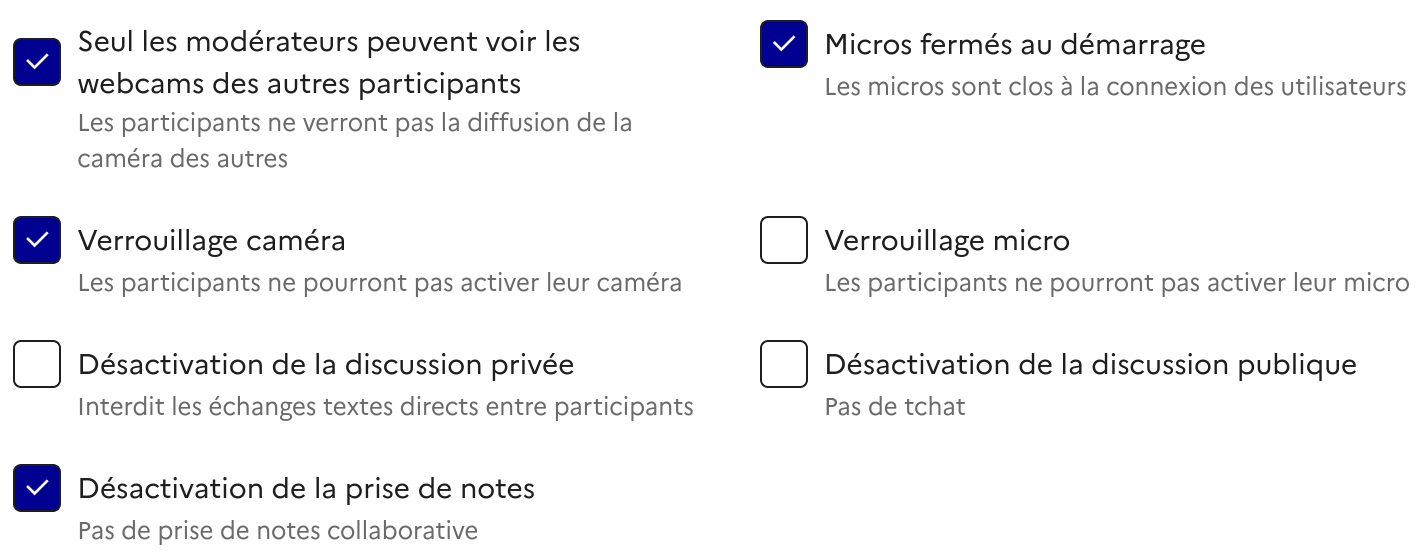
\includegraphics[width=11cm]{ressources/reglages.png}
              \captionof{figure}{Réglages}
              \label{reglages}
          \end{center}
    \item Enregistrer la configuration
\end{itemize}
\section{Partager l'adresse}
Afin de publier l'adresse du salon sur le site il faut que nous récupérions le lien dès maintenant.
\begin{itemize}
    \item Cliquer sur le bouton \emph{Inviter}
    \item Copier l'adresse \textbf{pour les participants}
    \item Se rendre sur \url{https://tinyurl.com/jpojay}
    \item Coller l'adresse en précisant la discipline
\end{itemize}
\section{Tester le salon}
Pour se familiariser avec l'environnement et voir les derniers réglages possibles, il faut ouvrir le salon.
\begin{itemize}
    \item Cliquer \emph{Lancer}
    \item Cliquer sur le microphone pour qu'un test soit lancé
    \item Autoriser l'utilisation du microphone par Firefox
    \item Les boutons en bas de l'écran permettent d'interagir avec les participants. Le bouton $\bigoplus$ permet par exemple de charger un pdf.
          \begin{center}
              \centering
              
\includegraphics[width=10cm]{ressources/boutons.png}
              \captionof{figure}{Interactions}
              \label{interagir}
          \end{center}
          Il faut garder en tête que le salon est un moment d'échanges avec les participants. Il peut être intéressant d'afficher une image synthétique de la discipline mais il semble peu pertinent de faire défiler un diaporama. De plus, cela influe sur la bande passante.
    
    \item Quelques réglages peuvent être effectués le jour de la présentation. Cliquer sur les trois points verticaux en haut à droite et choisir \emph{ouvrir les paramètres} (figure \ref{reg2})
    \item \begin{center}
        \centering
        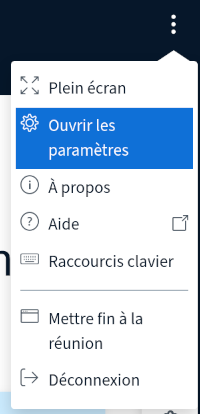
\includegraphics[width=3cm]{ressources/reglages2.png}
        \captionof{figure}{Options}
        \label{reg2}
    \end{center}
    
    \item Dans \emph{Applications} cocher \emph{Alertes Popup pour Nouveau participant}
    \item Si la réunion connaît des problèmes de bande-passante il faudra tout décocher dans \emph{Économies de données}
    \item Les invités arrivent dans une salle d'attente avant de pouvoir entrer dans le salon. C'est le modérateur qui autorise l'entrée.
\end{itemize}
\end{document}